\chapter{Demonstra\c{c}\~{a}o da Aplica\c{c}\~{a}o} \label{cap:demonstracao}

Este cap\'{i}tulo apresenta os principais fluxos da aplica\c{c}\~{a}o desenvolvida, com o objetivo de demonstrar o funcionamento das funcionalidades implementadas at\'{e} \`{a} fase atual do projeto. A demonstra\c{c}\~{a}o encontra-se organizada de acordo com o percurso natural de utiliza\c{c}\~{a}o da plataforma, desde a autentica\c{c}\~{a}o at\'{e} \`{a} gest\~{a}o e acompanhamento dos processos de averigua\c{c}\~{a}o.

\section{Autentica\c{c}\~{a}o e sele\c{c}\~{a}o de papel} \label{sec:demo-auth}

O primeiro contacto do utilizador com a aplica\c{c}\~{a}o ocorre atrav\'{e}s da p\'{a}gina de autentica\c{c}\~{a}o, representada na Figura~\ref{fig:demo-login}. Nesta p\'{a}gina, o utilizador introduz as suas credenciais para iniciar sess\~{a}o. Ap\'{o}s uma autentica\c{c}\~{a}o bem sucedida, a aplica\c{c}\~{a}o apresenta os pap\'{e}is dispon\'{i}veis para esse utilizador.

\begin{figure}[!htbp]
  \centering
  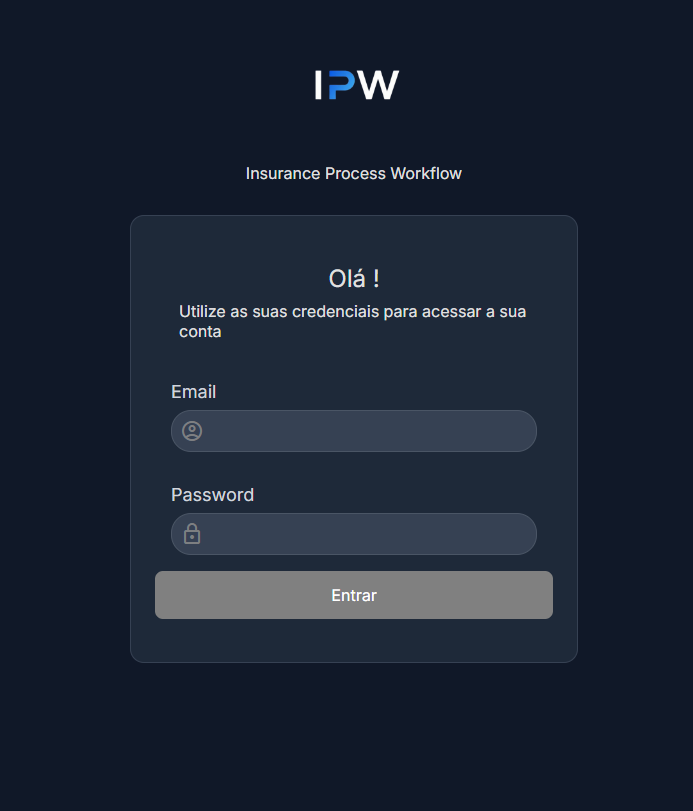
\includegraphics[height=0.30\textheight]{figures/novas/login_page.png}
  \caption{P\'{a}gina de autentica\c{c}\~{a}o da aplica\c{c}\~{a}o.}
  \label{fig:demo-login}
\end{figure}

A sele\c{c}\~{a}o de papel, apresentada na Figura~\ref{fig:demo-selecao-papel}, permite que o mesmo utilizador desempenhe diferentes fun\c{c}\~{o}es no sistema, quando aplic\'{a}vel. Esta decis\~{a}o define o contexto da sess\~{a}o e condiciona as funcionalidades dispon\'{i}veis na interface, bem como as rotas que podem ser acedidas no backend.

\begin{figure}[h]
  \centering
  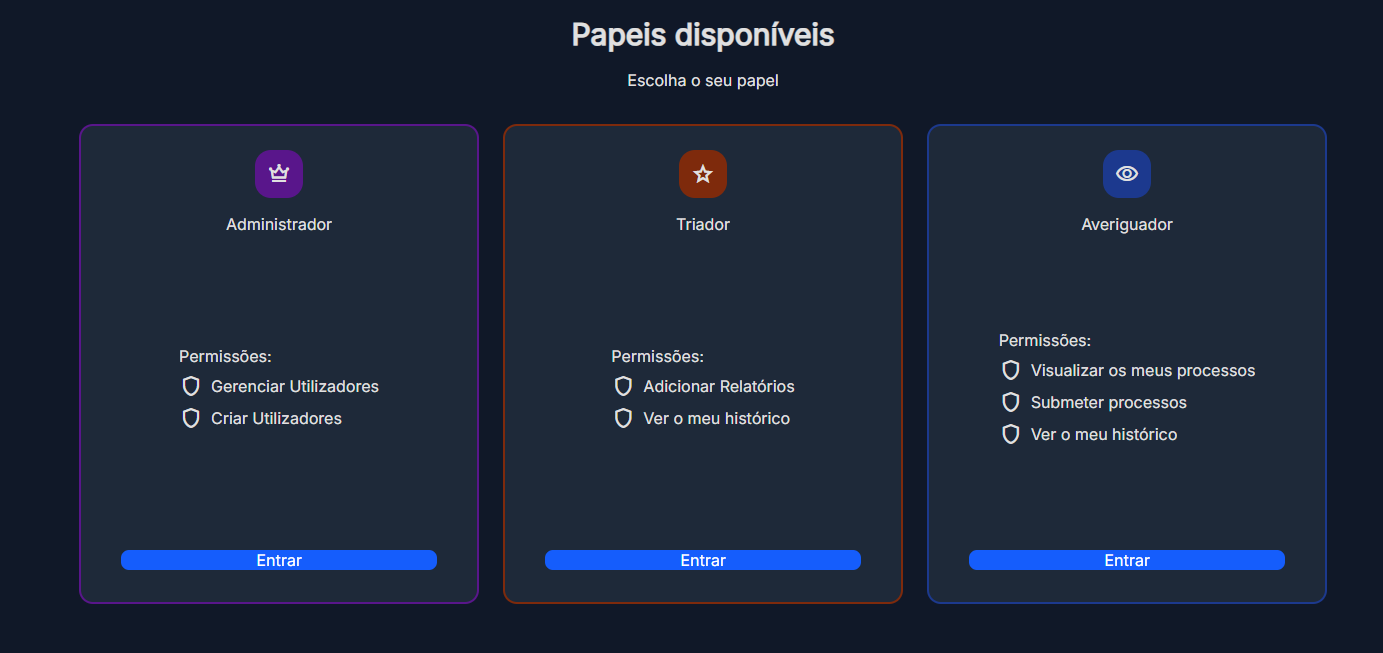
\includegraphics[width=0.85\textwidth]{figures/novas/role_selection.png}
  \caption{Sele\c{c}\~{a}o do papel ativo na sess\~{a}o do utilizador.}
  \label{fig:demo-selecao-papel}
\end{figure}

\section{Listagem e acompanhamento de processos} \label{sec:demo-processos}

Depois da sele\c{c}\~{a}o do papel, o utilizador \'{e} encaminhado para a \'{a}rea principal da aplica\c{c}\~{a}o, cujo conte\'{u}do varia consoante o papel selecionado. Para os pap\'{e}is diretamente envolvidos no acompanhamento de processos, esta \'{a}rea pode apresentar uma vis\~{a}o geral dos processos relevantes, como exemplificado na Figura~\ref{fig:demo-listagem-processos}, incluindo informa\c{c}\~{a}o resumida como o nome do processo, a localiza\c{c}\~{a}o, a \'{a}rea associada, a data limite e a prioridade.

\begin{figure}[h]
  \centering
  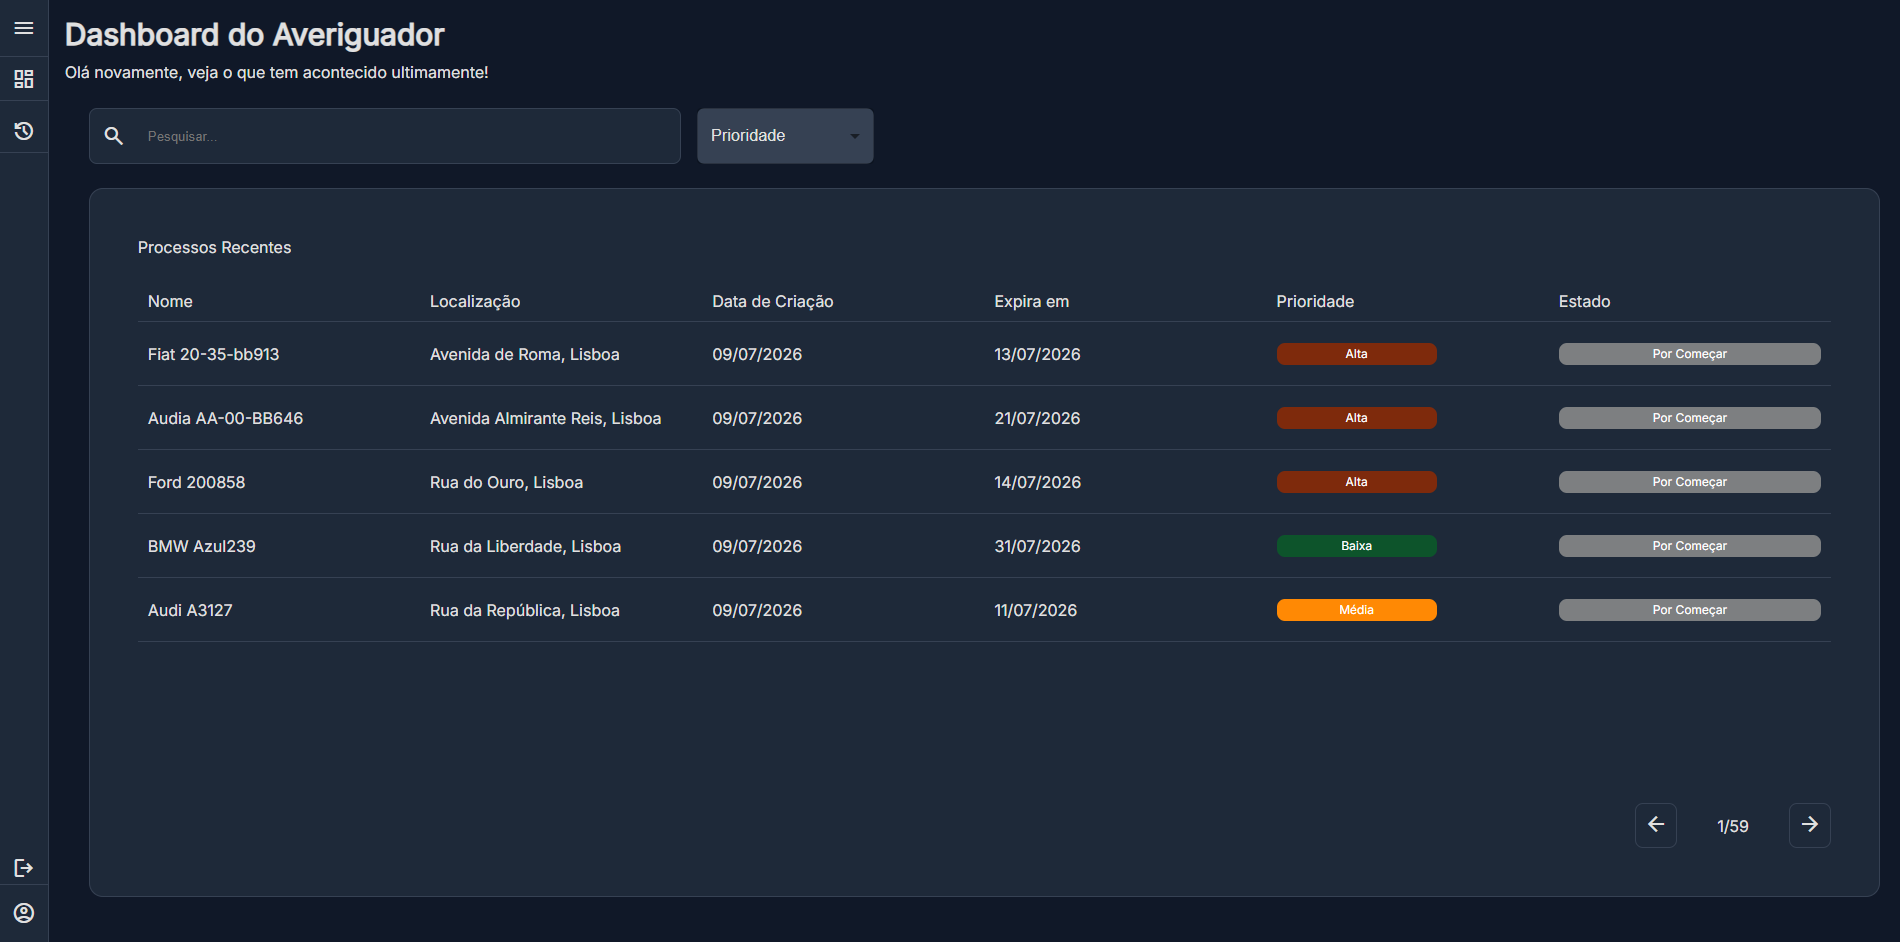
\includegraphics[width=0.95\textwidth]{figures/novas/dashboard_averiguador.png}
  \caption{Exemplo de listagem de processos dispon\'{i}vel para pap\'{e}is envolvidos no acompanhamento.}
  \label{fig:demo-listagem-processos}
\end{figure}

Quando dispon\'{i}vel, a tabela de processos serve como ponto de entrada para a consulta detalhada de cada processo. Esta abordagem permite que os utilizadores envolvidos no \textit{workflow} acompanhem o estado dos processos de forma centralizada, reduzindo a depend\^{e}ncia de informa\c{c}\~{a}o dispersa por diferentes ficheiros ou canais de comunica\c{c}\~{a}o.

\section{Cria\c{c}\~{a}o de processos} \label{sec:demo-criacao-processos}

A cria\c{c}\~{a}o de processos \'{e} uma funcionalidade associada ao papel de triador. Neste fluxo, representado na Figura~\ref{fig:demo-criacao-processo}, o triador preenche a informa\c{c}\~{a}o inicial do processo, incluindo dados como o nome, localiza\c{c}\~{a}o, \'{a}rea, prioridade, data limite, seguradora e tipifica\c{c}\~{a}o. Quando aplic\'{a}vel, o triador pode tamb\'{e}m atribuir manualmente um averiguador e um supervisor ao processo.

\begin{figure}[h]
  \centering
  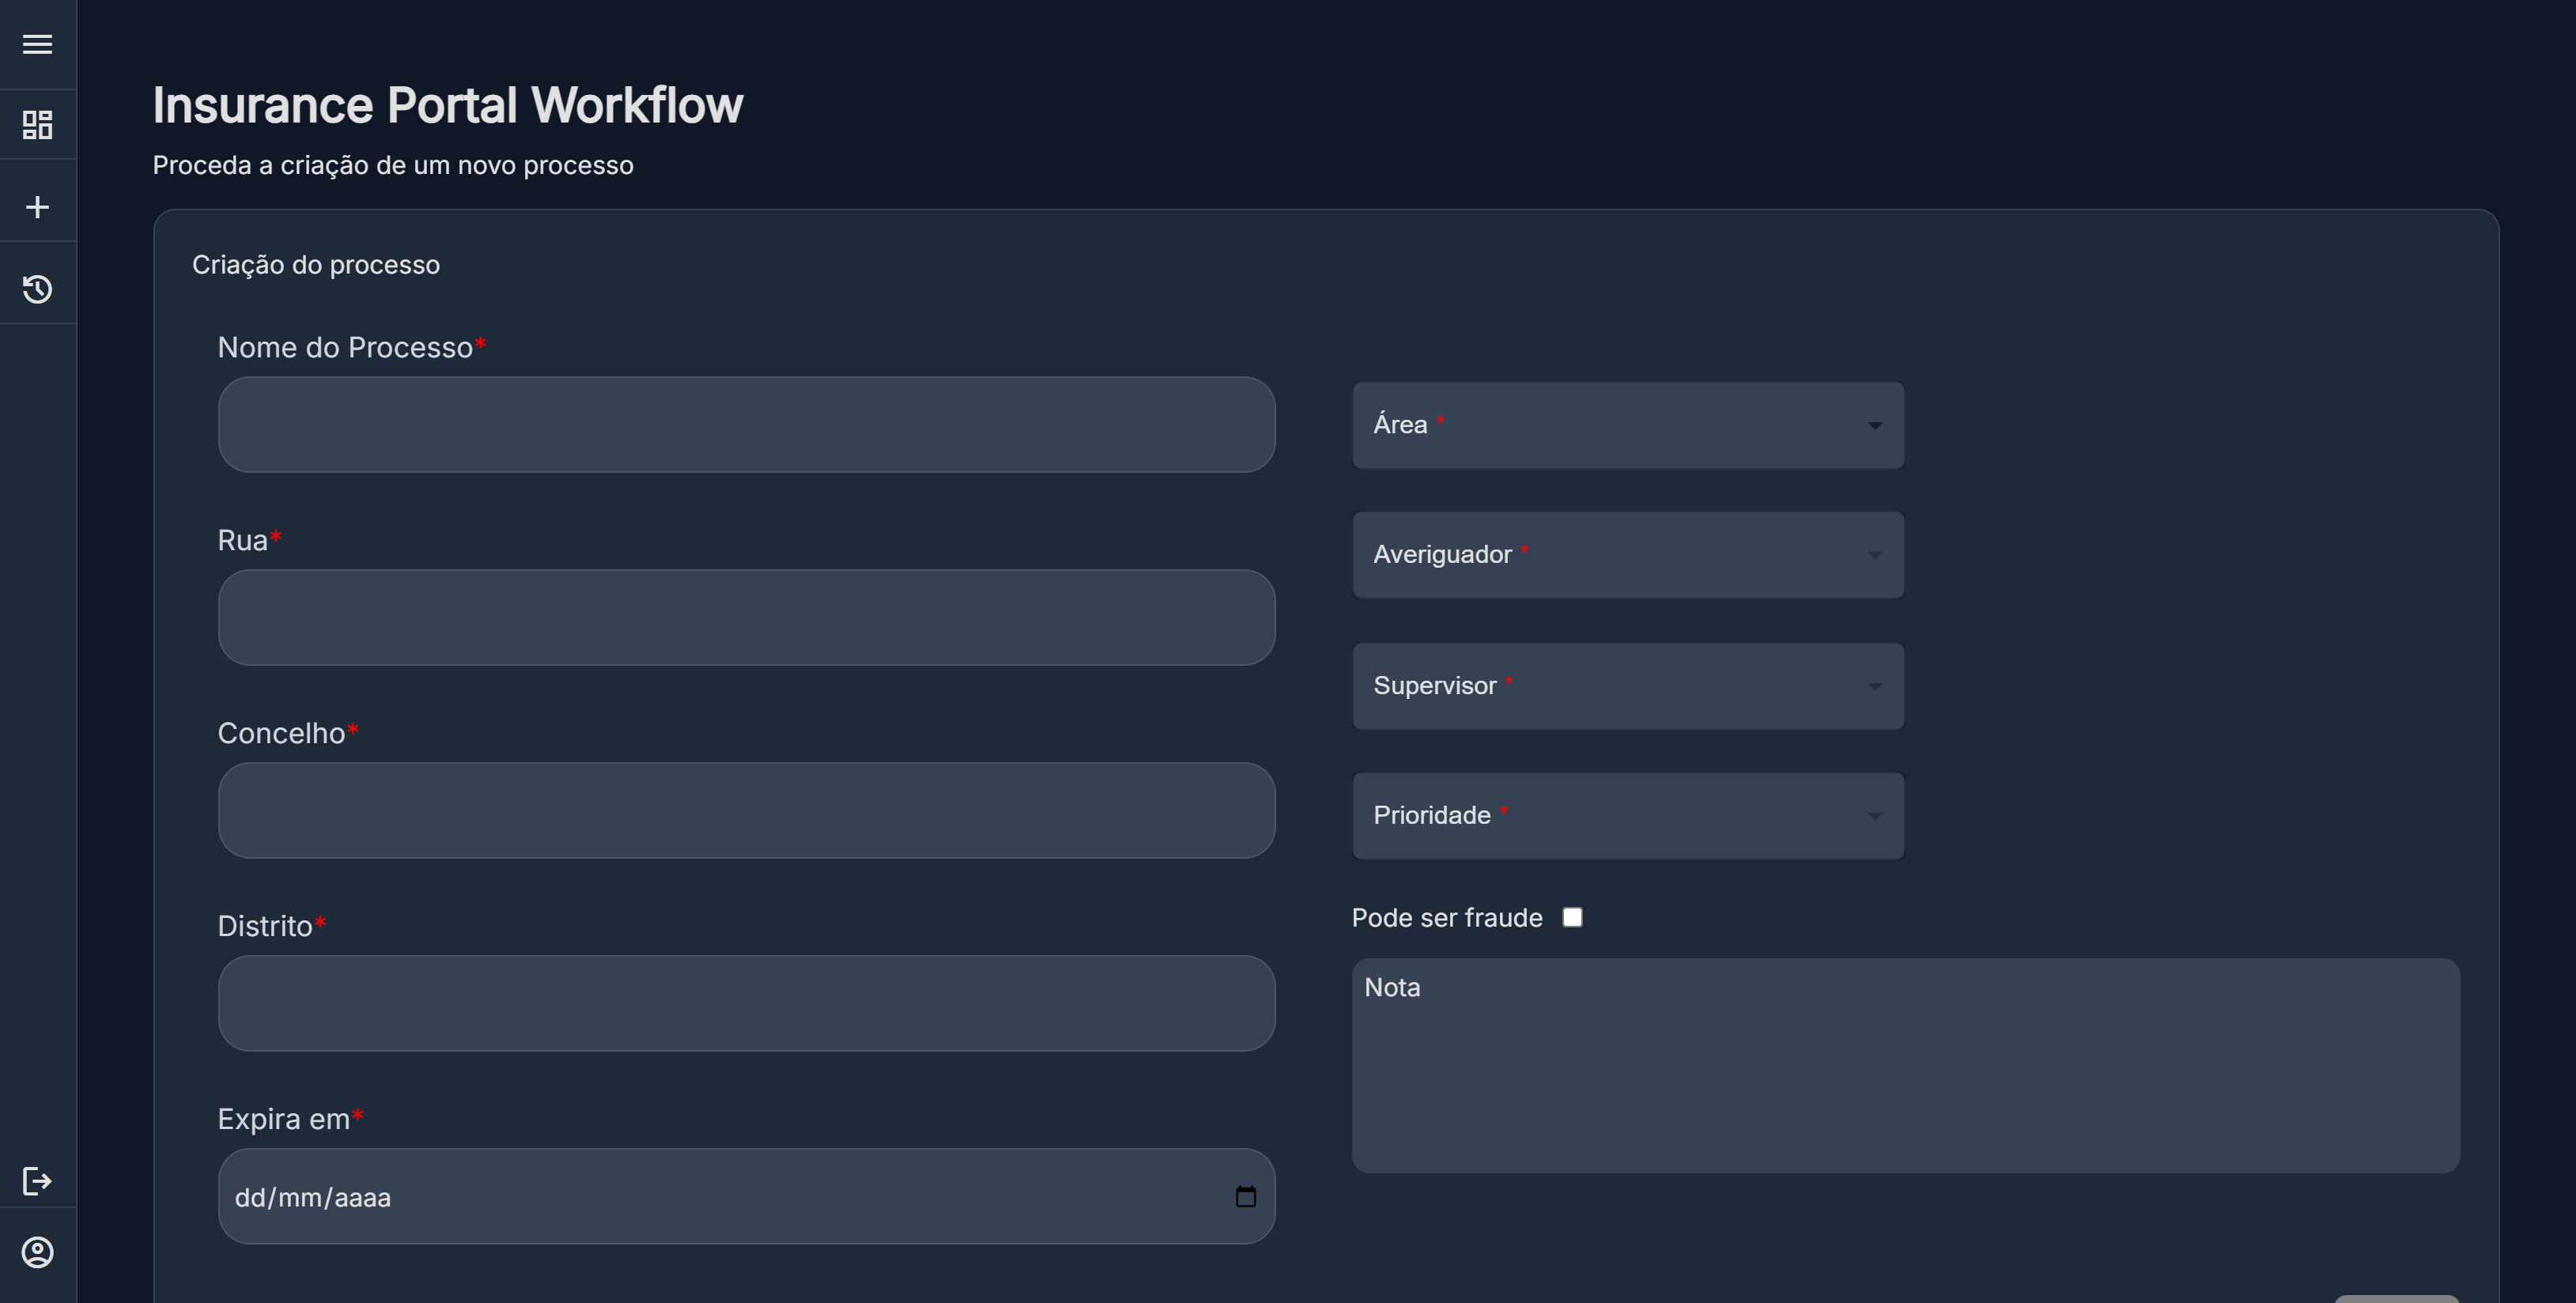
\includegraphics[width=0.95\textwidth]{figures/createProcess-page.png}
  \caption{Formul\'{a}rio de cria\c{c}\~{a}o de um novo processo pelo triador.}
  \label{fig:demo-criacao-processo}
\end{figure}

Este fluxo representa uma das funcionalidades centrais da aplica\c{c}\~{a}o, uma vez que formaliza a entrada de novos processos no sistema e permite associar, desde o in\'{i}cio, os intervenientes respons\'{a}veis pelo seu acompanhamento.

\section{Detalhe do processo} \label{sec:demo-detalhe-processo}

A p\'{a}gina de detalhe do processo, ilustrada na Figura~\ref{fig:demo-detalhe-processo}, disponibiliza informa\c{c}\~{a}o mais completa sobre um processo espec\'{i}fico. Nesta \'{a}rea s\~{a}o apresentados dados como os intervenientes atribu\'{i}dos, a \'{a}rea, datas relevantes, prioridade, estado atual e informa\c{c}\~{a}o associada ao relat\'{o}rio de averigua\c{c}\~{a}o.

\begin{figure}[h]
  \centering
  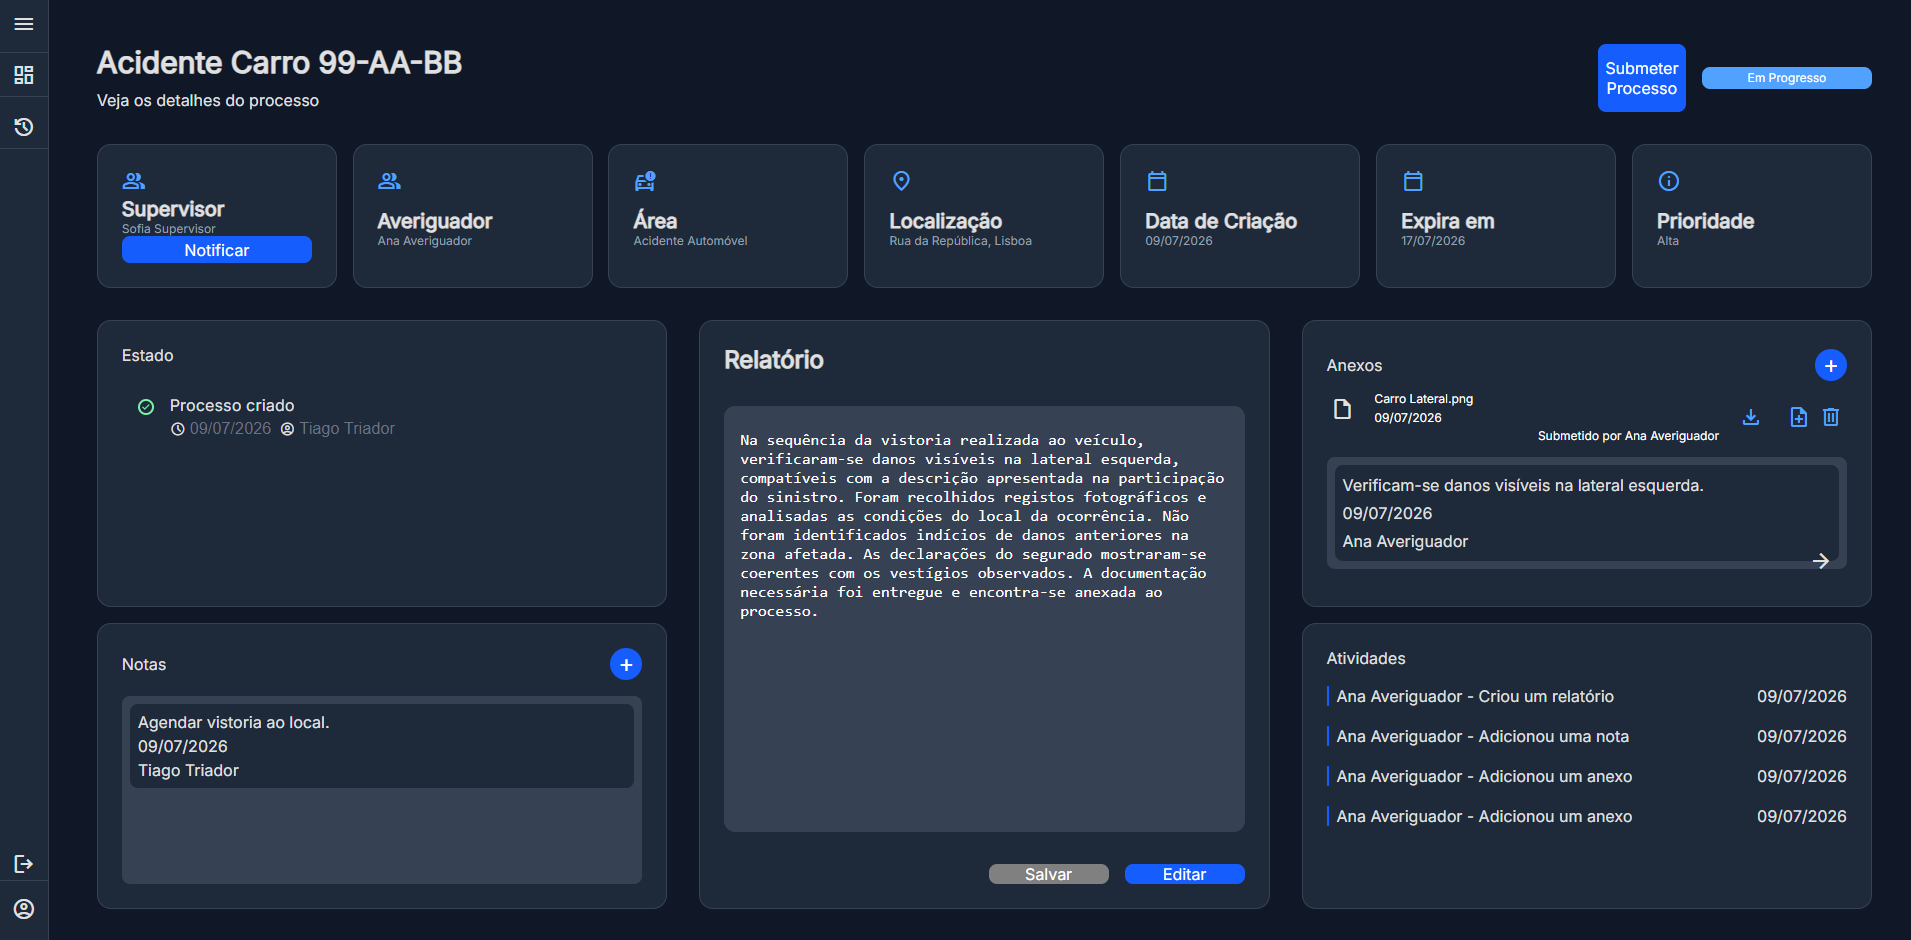
\includegraphics[width=0.95\textwidth]{figures/novas/process_view_investigator.png}
  \caption{P\'{a}gina de detalhe de um processo de averigua\c{c}\~{a}o.}
  \label{fig:demo-detalhe-processo}
\end{figure}

Esta p\'{a}gina permite concentrar num \'{u}nico local a informa\c{c}\~{a}o operacional do processo, facilitando o acompanhamento por parte dos diferentes pap\'{e}is envolvidos no \textit{workflow}.

\section{Gest\~{a}o de utilizadores} \label{sec:demo-users}

A aplica\c{c}\~{a}o inclui tamb\'{e}m funcionalidades de administra\c{c}\~{a}o, acess\'{i}veis a utilizadores com o papel de administrador. Atrav\'{e}s desta \'{a}rea, exemplificada na Figura~\ref{fig:demo-gestao-users}, \'{e} poss\'{i}vel consultar utilizadores, criar novos utilizadores, alterar pap\'{e}is e gerir a associa\c{c}\~{a}o de utilizadores a \'{a}reas.

\begin{figure}[h]
  \centering
  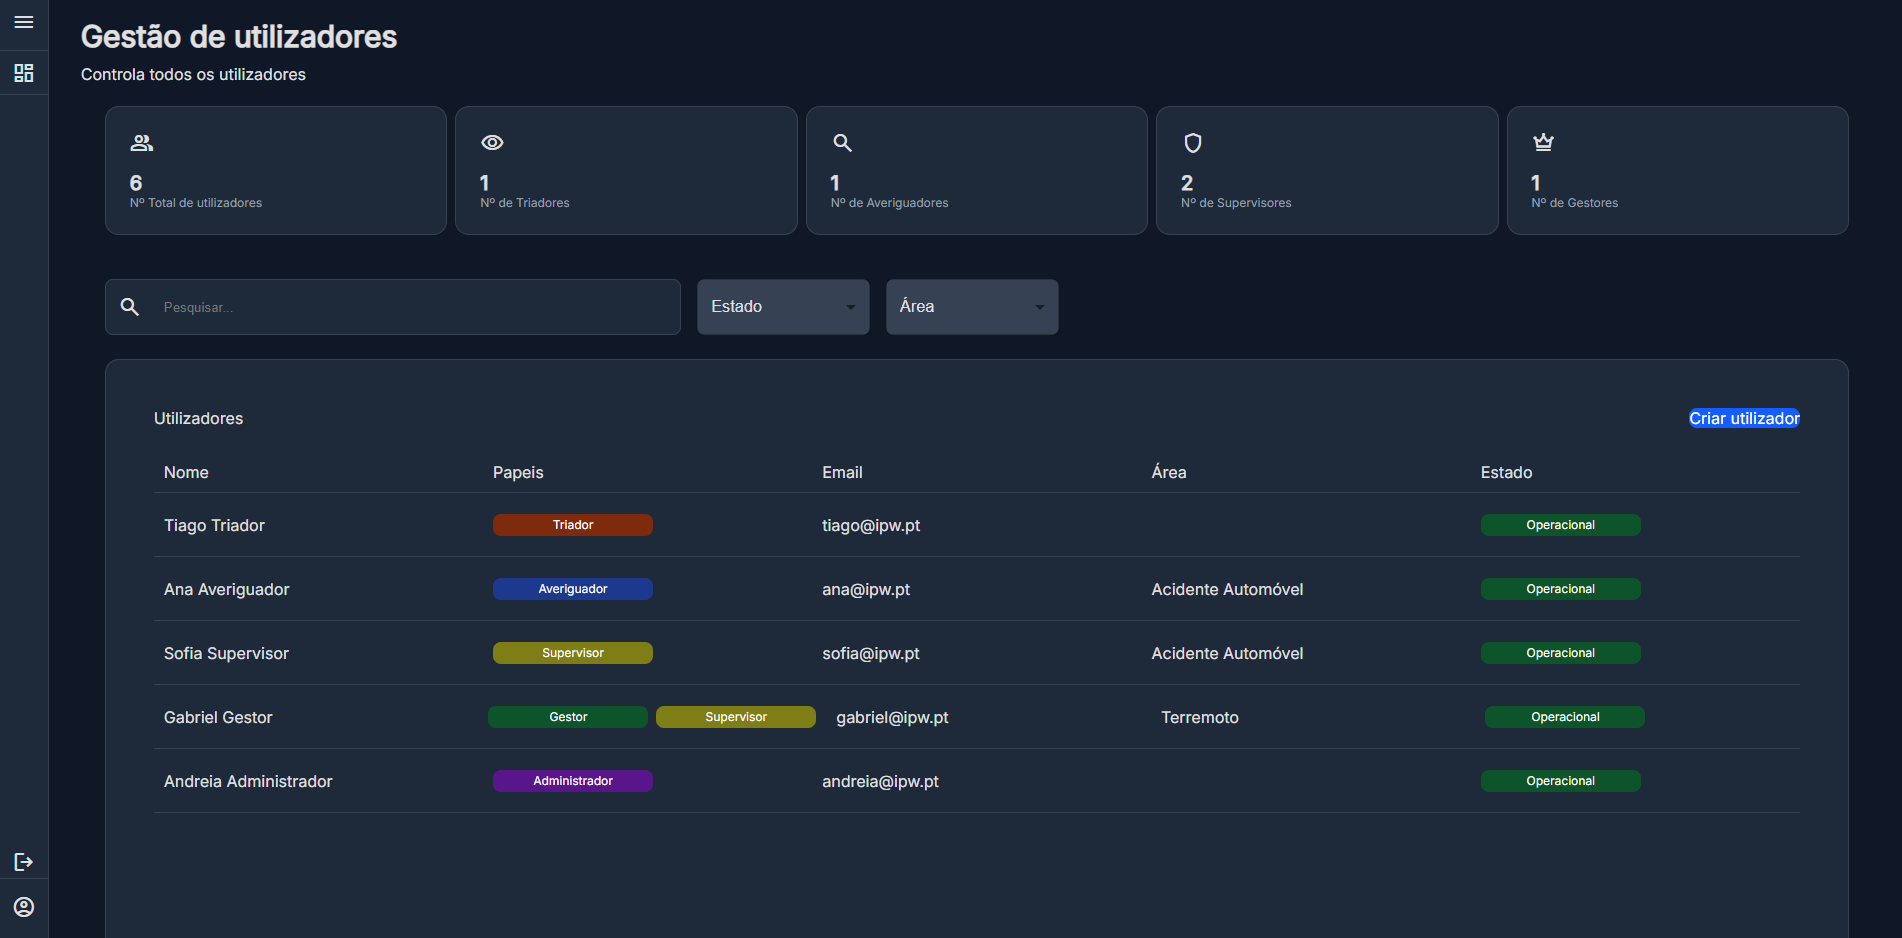
\includegraphics[width=0.95\textwidth]{figures/novas/admin_dashboard.png}
  \caption{Interface de gest\~{a}o de utilizadores dispon\'{i}vel ao administrador.}
  \label{fig:demo-gestao-users}
\end{figure}

Esta funcionalidade \'{e} relevante para manter o sistema alinhado com a organiza\c{c}\~{a}o interna da CAPT, permitindo refletir altera\c{c}\~{o}es nas equipas, responsabilidades e \'{a}reas de especializa\c{c}\~{a}o.

\section{Perfil e hist\'{o}rico de atividade} \label{sec:demo-perfil-historico}

Por fim, a aplica\c{c}\~{a}o disponibiliza uma \'{a}rea de perfil, onde o utilizador pode consultar informa\c{c}\~{a}o associada \`{a} sua conta e \`{a} sua atividade recente, como apresentado na Figura~\ref{fig:demo-perfil}. A exist\^{e}ncia de hist\'{o}rico e registo de intera\c{c}\~{o}es contribui para a rastreabilidade dos processos, permitindo perceber que opera\c{c}\~{o}es foram realizadas ao longo do tempo.

\begin{figure}[h]
  \centering
  
\includegraphics[width=0.95\textwidth]{figures/novas/profile_page.png}
  \caption{P\'{a}gina de perfil e consulta de atividade recente do utilizador.}
  \label{fig:demo-perfil}
\end{figure}

Em conjunto, estes fluxos demonstram a base funcional da plataforma \textit{IPW} e a forma como a aplica\c{c}\~{a}o suporta a gest\~{a}o estruturada dos processos de averigua\c{c}\~{a}o.
